\section{Kernel audits, head-to-head benchmarks and weak rates}
\label{sec:benchmarks}

We now address three questions faced by volatility desks and model validators: (i) how large the continuous-time kernel-approximation error of Markovian and hybrid schemes can be, certified in Arb (Experiment~E3); (ii) how six published SPX pricing families compare against a continuum enclosure in three market regimes (Experiment~E4); and (iii) how measured weak rates compare with $\beta_{\mathrm{FSW}}(H)$ and with the Jensen-$J$ ablation of Proposition~\ref{prop:jensen_pitfall} (Experiment~E5).

\subsection{Experiment E3: continuous-time kernel audit in Arb}
\label{sec:e3}

Before any Markovian or hybrid simulation, Theorem~\ref{thm:put_lipschitz} bounds the continuous-time kernel gap $|C(K)-C_{\hat{K}}(K)|$ in Arb. We audit \citet{BayerBreneis2023} exponential sums fitted by unclipped, preconditioned L-BFGS-B ($M\in\{2,4,6,8,12,16\}$ factors, $H\in\{0.07,0.10,0.30\}$) and \citet{BennedsenLundePakkanen2017} hybrid kernels ($\kappa\in\{1,2,3,4,6,8\}$, $n=256$) on calibrated rough Bergomi ($T=0.25$, $\eta=1.9$, $\rho=-0.9$, $\xi_0=0.04$). At $H=0.10$ the empirical errors are measured against a $131{,}072$-path \RCBridge{} reference on levels $(64,128,256,512)$ with ATM implied volatility $[\EThreeRefATMLo,\EThreeRefATMHi]\%$ (width $\EThreeRefATMW\bps$) and finite-difference ATM skew $[\EThreeRefSkewLo,\EThreeRefSkewHi]$ ($\delta k=0.02$). Table~\ref{tab:e3_kernel} and Figure~\ref{fig:e3_kernel} summarise the results.

\begin{table}[t]
\centering
\caption{\ArbBits-bit Arb continuous-time kernel audit at $H=0.10$, $T=0.25$, $\eta=1.9$, $\rho=-0.9$, $\xi_0=0.04$.}
\label{tab:e3_kernel}
\footnotesize
\setlength{\tabcolsep}{4.0pt}
\begin{tabular}{@{}lrrrrrrr@{}}
\toprule
Kernel approximation & $\|K{-}\hat{K}\|_{L^2}$ & $\|K{-}\hat{K}\|_{L^1}$ & $E_J$ upper & Price gap & Fit & ATM IV err & Emp.\ ATM \\
 & (Arb) & (Arb) & (Arb) & (Arb) & (s) & (bps, stat.) & skew \\
\midrule
BB2023 ($M=2$) & 0.3254 & 0.05556 & 0.02989 & 0.03452 & 0.13 & $[12.6,\,21.5]$ & $-0.6117$ \\
BB2023 ($M=4$) & 0.1747 & 0.02805 & 0.01622 & 0.01873 & 0.19 & $[0.0,\,5.8]$ & $-0.5985$ \\
BB2023 ($M=6$) & 0.1044 & 0.01584 & 0.00973 & 0.01124 & 0.35 & $[0.0,\,7.2]$ & $-0.5932$ \\
BB2023 ($M=8$) & 0.0665 & 0.00957 & 0.00621 & 0.00717 & 0.51 & $[0.0,\,8.6]$ & $-0.5919$ \\
BB2023 ($M=12$) & 0.0304 & 0.00402 & 0.00285 & 0.00329 & 1.03 & $[0.0,\,5.1]$ & $-0.5944$ \\
BB2023 ($M=16$) & 0.0155 & 0.00192 & 0.00145 & 0.00168 & 2.80 & $[0.0,\,4.6]$ & $-0.5948$ \\
\midrule
BLP hybrid ($\kappa=1$, $n=256$) & -- & -- & 0.00175 & 0.00202 & -- & $\le 101.0^{\ddagger}$ & -- \\
BLP hybrid ($\kappa=2$, $n=256$) & -- & -- & 0.00096 & 0.00111 & -- & $\le 55.6^{\ddagger}$ & -- \\
BLP hybrid ($\kappa=4$, $n=256$) & -- & -- & 0.00052 & 0.00060 & -- & $\le 29.9^{\ddagger}$ & -- \\
BLP hybrid ($\kappa=8$, $n=256$) & -- & -- & 0.00028 & 0.00032 & -- & $\le 15.8^{\ddagger}$ & -- \\
\bottomrule
\end{tabular}
\par\smallskip
\parbox{\linewidth}{\footnotesize\emph{Notes.} Upper panel: unclipped L-BFGS-B factors of \citet{BayerBreneis2023}; columns 2--5 are Arb-certified upper bounds; the ATM error interval ($n=256$) is statistical, against the \RCBridge{} reference ATM IV $[\EThreeRefATMLo,\EThreeRefATMHi]\%$. Lower panel: continuous-time hybrid kernel. $^{\ddagger}$Certified gap mapped to IV across the statistical reference bracket (conditional; time stepping excluded).}
\end{table}
%

\begin{figure}[t]
  \centering
  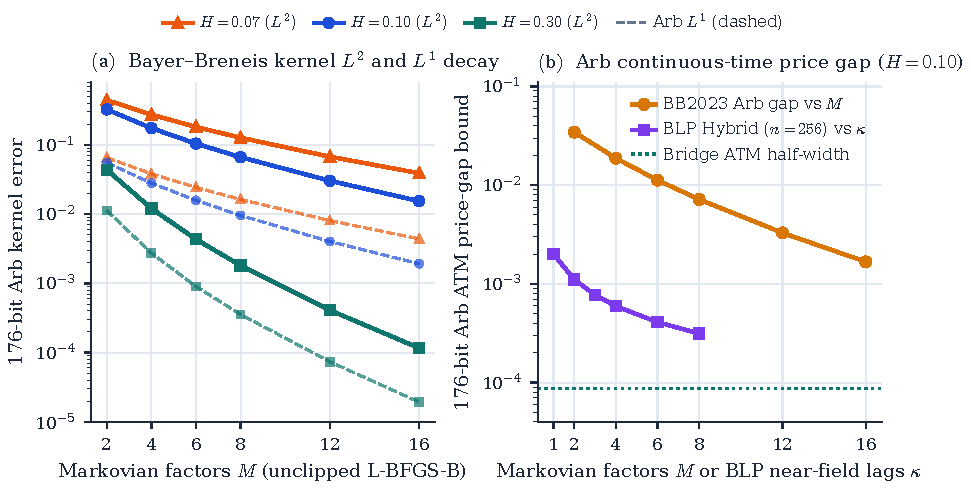
\includegraphics[width=\textwidth]{figures/fig_e3_kernel_audit.pdf}
  \caption{Continuous-time kernel audit in Arb ($T=0.25$, $\eta=1.9$, $\rho=-0.9$, $\xi_0=0.04$). (a) Certified $L^2$ (solid) and root-splitting $L^1$ (dashed) errors of unclipped \citet{BayerBreneis2023} kernels for $H\in\{0.07,0.10,0.30\}$. (b) Certified ATM price-gap bounds for Markovian factors $M$ and hybrid lags $\kappa$ at $H=0.10$.}
  \label{fig:e3_kernel}
\end{figure}

Three findings bear on kernel selection.
\begin{enumerate}[1.]
  \item \emph{Geometric decay of the Markovian kernel error.} Without artificial upper bounds on the mean-reversion speeds $x_j$, which stall the decay at small $H$, the certified $L^2$ error at $H=0.10$ falls from $\EThreeMkTenMTwoLTwo$ ($M=2$) to $\EThreeMkTenMSixteenLTwo$ ($M=16$, fit time $\EThreeMkTenMSixteenFit\,\mathrm{s}$), and the certified $L^1$ error reaches $\EThreeMkTenMSixteenLOne$. With $M=16$ the certified $L^2$ error is $\EThreeMkSevenMSixteenLTwo$ at $H=0.07$ and $\EThreeMkThirtyMSixteenLTwo$ at $H=0.30$.
  \item \emph{The price-gap certificate is conservative at calibrated vol-of-vol.} At $H=0.10$ and $M=16$, Theorem~\ref{thm:put_lipschitz} bounds the continuous-time ATM price gap by $\EThreeMkTenMSixteenGap$, about $\EThreeMkTenMSixteenGapIV\bps$ in implied volatility, whereas the empirical ATM IV error against \RCBridge{} is at most $\EThreeMkTenMSixteenATMHi\bps$, smaller by a factor of at least $\EThreeMkGapOverEmp$. The bound is first order in $E_J$ and admits no cancellation; its value lies in holding before any simulation and in decaying geometrically with $M$ (about $\EThreeMkTenMTwelveGapIV\bps$ at $M=12$). The empirical ATM error interval itself contracts from at least $\EThreeMkTenMTwoATMLo\bps$ ($M=2$) to at most $\EThreeMkTenMSixteenATMHi\bps$ ($M=16$).
  \item \emph{Hybrid kernel gap.} Propagating the certified continuous-time hybrid price gap across the statistical reference ATM price bracket bounds the IV gap by $\EThreeBLPKapOneIV\bps$ ($\kappa=1$), $\EThreeBLPKapTwoIV\bps$ ($\kappa=2$), $\EThreeBLPKapFourIV\bps$ ($\kappa=4$) and $\EThreeBLPKapEightIV\bps$ ($\kappa=8$) at $n=256$. These IV figures inherit the statistical status of the reference bracket, and they exclude discrete time-stepping error by construction. A code-disjoint evaluation of $E_J$ for the hybrid kernels lies inside every stored Arb ball (check~I3).
\end{enumerate}

\subsection{Experiment E4: head-to-head SPX benchmarks in three regimes}
\label{sec:e4}

We benchmark six published SPX rough-Bergomi pricing families on identical single-threaded hardware, reporting \emph{cold setup time} and \emph{amortised solve time} separately, with error intervals $[\operatorname{dist}(v,[L,U]),\max(|v-L|,|v-U|)]$ against a $131{,}072$-path \RCBridge{} reference on levels $(64,128,256,512)$:
\begin{itemize}
  \item \emph{Regime~A (calibrated three-month SPX):} $H=0.10$, $T=0.25$, $\eta=1.9$, $\rho=-0.9$, $\xi_0=0.04$, eight strikes in $[0.85,1.12]$ including the skew stencil $e^{\pm 0.02}$; reference ATM IV $[\EFourARefATMLo,\EFourARefATMHi]\%$ (width $\EFourARefATMW\bps$, $\EFourARefDiag$ diagnostic strike at $K=0.85$) and ATM skew $[\EFourARefSkewLo,\EFourARefSkewHi]$.
  \item \emph{Regime~B (ultra-rough one-month SPX):} $H=0.07$, $T=1/12$, $\eta=1.9$, $\rho=-0.9$, $\xi_0=0.235^2$, seven strikes in $[0.90,1.08]$ including $e^{\pm 0.015}$; reference ATM IV $[\EFourBRefATMLo,\EFourBRefATMHi]\%$ (width $\EFourBRefATMW\bps$, $\EFourBRefDiag$ diagnostic strikes at $K\in\{0.95,1.05\}$) and ATM skew $[\EFourBRefSkewLo,\EFourBRefSkewHi]$.
  \item \emph{Regime~C (curved forward variance, six months):} $H=0.10$, $T=0.50$, $\eta=1.9$, $\rho=-0.85$, $\xi_0(t)=0.234^2(1+t)^2$, seven strikes in $[0.80,1.20]$ including $e^{\pm 0.02}$; reference ATM IV $[\EFourCRefATMLo,\EFourCRefATMHi]\%$ (width $\EFourCRefATMW\bps$, no diagnostic strike) and ATM skew $[\EFourCRefSkewLo,\EFourCRefSkewHi]$.
\end{itemize}
Every simulated competitor uses the same main budget of $32{,}768$ paths ($R=16$ shifts of $2{,}048$ antithetic paths) and a sampling-type label. Scrambled Sobol RQMC with the pilot-fitted control bank ($R_{\mathrm{pilot}}=2$ extra pilot shifts, timed inside the solve time) is used for \RCCE{} and for the Brownian-bridge left-point RQMC of \citet{BayerBenHammoudaTempone2020}, whose Richardson extrapolation is labelled \emph{diagnostic}. Pseudo-random antithetic MC with Romano--Touzi conditioning and two-control leave-one-shift-out cross-fitting is used for the hybrid scheme of \citet{McCrickerdPakkanen2018} ($\kappa\in\{1,2\}$), the Markovian scheme of \citet{BayerBreneis2023} and the rDonsker scheme of \citet{HorvathJacquierMuguruza2024}, whose Eq.~(4.2) gives the variance-matched (vm) cell weight $(\Delta t^{-1}\int_{\rm cell}K_H^2)^{1/2}$. Our comparison also uses the cell mean $\Delta t^{-1}\int_{\rm cell}K_H$, the $L^2$ projection evaluated at the optimal point $b_k^*$ of \citet{BennedsenLundePakkanen2017}. The order-two expansion of \citet{BergomiGuyon2012} is analytic and labelled \emph{diagnostic}. In tables and figures these competitors appear as BHT2020, MP2018, BB2023, HJMS2024 and BG2012. The simulated methods share common random numbers, which sharpens comparisons without affecting the validity of each marginal interval (\ref{app:repro}). Tables~\ref{tab:e4_regimeA}--\ref{tab:e4_regimesBC} and Figures~\ref{fig:e4_dot}--\ref{fig:e4_wp} report the results.

\begin{table}[t]
\centering
\caption{Head-to-head SPX benchmarks in Regime~A ($H=0.10$, $T=0.25$, $\eta=1.9$, $\rho=-0.9$, $\xi_0=0.04$, $8$ strikes in $[0.85,1.12]$).}
\label{tab:e4_regimeA}
\footnotesize
\setlength{\tabcolsep}{3.6pt}
\begin{tabular}{@{}llrrrrrr@{}}
\toprule
Method & Type & Setup & Solve & ATM IV err & Max smile err & ATM & Skew err \\
($32{,}768$ paths; 1 thread) & & (s) & (s) & (bps) & (bps) & skew & interval \\
\midrule
\RCCE{} ($n=128$) & RQMC & 0.06 & 2.27 & $[0.0,\,7.7]$ & $[0.0,\,67.8]$ & $-0.590$ & $[0.000,\,0.056]$ \\
\RCCE{} ($n=256$) & RQMC & 0.38 & 4.80 & $[0.0,\,7.8]$ & $[0.0,\,55.5]$ & $-0.594$ & $[0.000,\,0.052]$ \\
Jensen-$J$ ablation ($n=256$) & RQMC & 0.38 & 9.48 & $[3.9,\,17.4]$ & $[3.9,\,57.9]$ & $-0.590$ & $[0.000,\,0.056]$ \\
BHT2020 Bridge-RQMC ($n=128$) & RQMC & 0.01 & 1.87 & $[0.0,\,7.2]$ & $[2.1,\,83.6]$ & $-0.589$ & $[0.000,\,0.057]$ \\
BHT2020 Bridge-RQMC ($n=256$) & RQMC & 0.06 & 3.59 & $[0.0,\,8.8]$ & $[0.0,\,61.9]$ & $-0.590$ & $[0.000,\,0.056]$ \\
BHT2020 Richardson (64,128) & Diag. & 0.01 & 2.87 & $[0.0,\,8.2]$ & $[0.9,\,66.9]$ & $-0.608$ & $[0.000,\,0.059]$ \\
MP2018 hybrid ($\kappa=1,n=128$) & MC & 0.00 & 0.88 & $[0.0,\,7.0]$ & $[2.6,\,82.5]$ & $-0.585$ & $[0.000,\,0.061]$ \\
MP2018 hybrid ($\kappa=2,n=256$) & MC & 0.01 & 2.26 & $[0.0,\,6.9]$ & $[0.0,\,61.6]$ & $-0.594$ & $[0.000,\,0.051]$ \\
BB2023 Markov ($M=8,n=128$) & MC & 0.57 & 2.15 & $[0.0,\,7.4]$ & $[0.8,\,80.7]$ & $-0.588$ & $[0.000,\,0.058]$ \\
BB2023 Markov ($M=12,n=256$) & MC & 1.10 & 5.32 & $[0.0,\,13.2]$ & $[0.0,\,67.8]$ & $-0.587$ & $[0.000,\,0.059]$ \\
HJMS2024 rDonsker (vm, $n=256$) & MC & 0.00 & 1.74 & $[5.5,\,19.1]$ & $[7.6,\,59.8]$ & $-0.614$ & $[0.000,\,0.065]$ \\
rDonsker (BLP $b_k^*$, $n=256$) & MC & 0.00 & 1.76 & $[2.0,\,15.6]$ & $[34.2,\,115.7]$ & $-0.624$ & $[0.000,\,0.074]$ \\
BG2012 order-2 expansion & Diag. & 0.00 & 0.00 & $[42.9,\,56.5]$ & $[295.4,\,376.9]$ & $-0.681$ & $[0.036,\,0.132]$ \\
\bottomrule
\end{tabular}
\par\smallskip
\parbox{\linewidth}{\footnotesize\emph{Notes.} Errors: $[\operatorname{dist}(v,[L,U]),\max(|v-L|,|v-U|)]$ for the point estimate $v$ against the $131{,}072$-path \RCBridge{} reference (ATM IV $[\EFourARefATMLo,\EFourARefATMHi]\%$, skew $[\EFourARefSkewLo,\EFourARefSkewHi]$); the sampling error of $v$ is not included. Type: scrambled-Sobol RQMC, pseudo-random MC, analytic or diagnostic. Simulated methods share common random numbers.}
\end{table}
%

\begin{figure}[t]
  \centering
  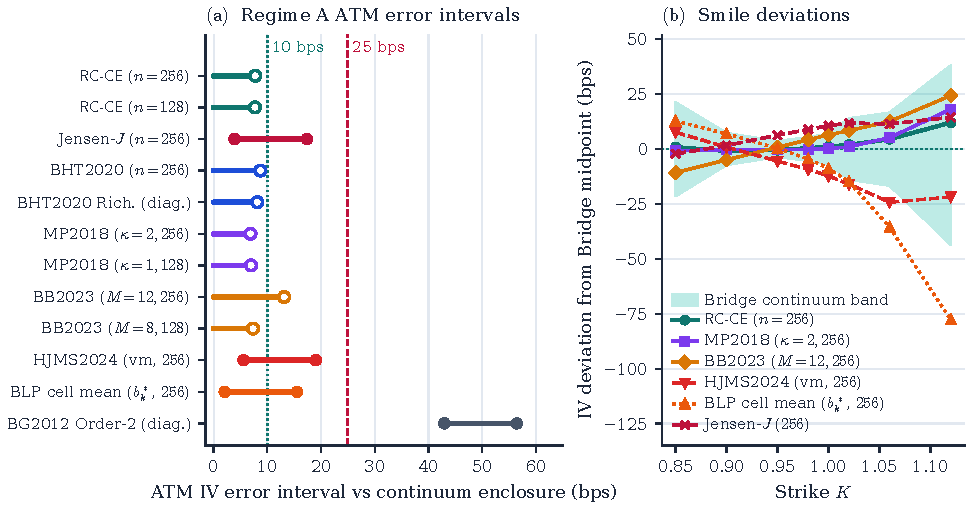
\includegraphics[width=\textwidth]{figures/fig_e4_dot_table.pdf}
  \caption{Head-to-head SPX benchmarks in Regime~A ($H=0.10$, $T=0.25$, $\eta=1.9$, $\rho=-0.9$). (a) ATM IV error intervals against the $131{,}072$-path \RCBridge{} enclosure; open circles mark zero lower distance. (b) Signed smile deviations from the Bridge midpoint across $K\in[0.85,1.12]$.}
  \label{fig:e4_dot}
\end{figure}

\begin{figure}[t]
  \centering
  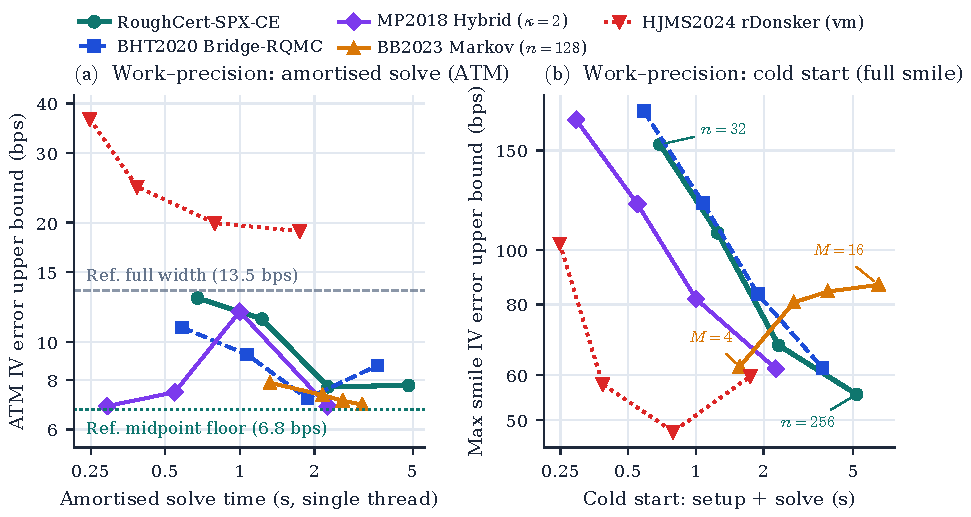
\includegraphics[width=\textwidth]{figures/fig_e4_work_precision.pdf}
  \caption{Work--precision curves in Regime~A ($32{,}768$ paths, one thread). (a) Upper end of the ATM IV error against amortised solve time, with the reference midpoint floor $W/2$. (b) Upper end of the maximum smile IV error over $K\in[0.85,1.12]$ against cold-start time (setup plus solve).}
  \label{fig:e4_wp}
\end{figure}

\begin{table}[t]
\centering
\caption{Head-to-head benchmarks in Regime~B (ultra-rough one-month, $H=0.07$) and Regime~C (curved $\xi_0(t)$, $T=0.50$).}
\label{tab:e4_regimesBC}
\footnotesize
\begin{tabular}{@{}llrrrr@{}}
\toprule
Regime and method & Type & Solve (s) & ATM IV err (bps) & Max smile err (bps) & ATM skew \\
\midrule
B: \RCCE{} ($n=128$) & RQMC & 2.32 & $[0.0,\,7.6]$ & $[0.0,\,91.3]$ & $-0.865$ \\
B: BHT2020 ($n=128$) & RQMC & 2.48 & $[0.0,\,9.4]$ & $[1.7,\,91.9]$ & $-0.866$ \\
B: MP2018 ($\kappa=2,n=128$) & MC & 1.38 & $[0.0,\,8.4]$ & $[2.4,\,95.2]$ & $-0.863$ \\
B: BB2023 ($M=12,n=128$) & MC & 3.10 & $[0.0,\,9.2]$ & $[0.8,\,89.3]$ & $-0.874$ \\
B: HJMS2024 (vm, $n=128$) & MC & 0.79 & $[13.4,\,27.4]$ & $[19.1,\,121.3]$ & $-0.944$ \\
B: BG2012 order-2 & Diag. & 0.00 & $[34.0,\,48.1]$ & $[276.1,\,358.2]$ & $-1.030$ \\
\midrule
C: \RCCE{} ($n=128$) & RQMC & 3.07 & $[0.0,\,9.4]$ & $[0.0,\,51.4]$ & $-0.426$ \\
C: BHT2020 ($n=128$) & RQMC & 2.54 & $[0.0,\,8.0]$ & $[0.0,\,67.1]$ & $-0.423$ \\
C: MP2018 ($\kappa=2,n=128$) & MC & 1.42 & $[0.0,\,8.2]$ & $[5.0,\,76.0]$ & $-0.421$ \\
\bottomrule
\end{tabular}
\par\smallskip
\parbox{\linewidth}{\footnotesize\emph{Notes.} Regime~B ($H=0.07$, $T=1/12$, $\eta=1.9$, $\rho=-0.9$, $\xi_0=0.235^2$): \RCBridge{} ATM IV $[\EFourBRefATMLo,\EFourBRefATMHi]\%$, skew $[\EFourBRefSkewLo,\EFourBRefSkewHi]$. Regime~C ($H=0.10$, $T=0.50$, $\eta=1.9$, $\rho=-0.85$, $\xi_0(t)=0.234^2(1+t)^2$): ATM IV $[\EFourCRefATMLo,\EFourCRefATMHi]\%$, skew $[\EFourCRefSkewLo,\EFourCRefSkewHi]$. Error intervals as in Table~\ref{tab:e4_regimeA}.}
\end{table}
%

Five lessons emerge across Regimes~A--C.
\begin{enumerate}[1.]
  \item \emph{Exact-grid \RCCE{} and BHT2020 track the reference closely.} In Regime~A, the ATM IV error of \RCCE{} is at most $\EFourACEOneTwoEightATMHi\bps$ at $n=128$ and $\EFourACETwoFiveSixATMHi\bps$ at $n=256$ (solve time $\EFourACETwoFiveSixSolve\,\mathrm{s}$), with zero lower distance across the smile core. The Jensen-$J$ ablation at $n=256$ behaves differently: its 95\% confidence interval at the money lies $\EFourAJenTwoFiveSixATMCIDist\bps$ above the reference envelope, and its point estimate is at least $\EFourAJenTwoFiveSixMaxLo\bps$ from the envelope somewhere on the smile, consistent with Proposition~\ref{prop:jensen_pitfall}.
  \item \emph{The MP2018 hybrid scheme ($\kappa=2$) is fastest after amortisation, but its bias needs an external audit.} It solves in $\EFourAMPTwoTwoFiveSixSolve\,\mathrm{s}$ at $n=256$ ($\EFourAMPTwoOneTwoEightSolve\,\mathrm{s}$ at $n=128$) with ATM error at most $\EFourAMPTwoTwoFiveSixATMHi\bps$. A single-grid run does not bound its own time-step bias; that requires an \RCBridge{} or Arb kernel audit.
  \item \emph{The unclipped BB2023 Markovian scheme ($M=12$) is accurate once its setup is amortised.} After the $\EFourABBMTwelveSetup\,\mathrm{s}$ one-time kernel fit, it solves in $\EFourABBMTwelveSolveTwoFiveSix\,\mathrm{s}$ at $n=256$ with zero lower distance across the smile. At $n=128$ (Figure~\ref{fig:e4_wp}(b)), increasing $M$ from $4$ to $16$ slightly raises the upper smile error, which we attribute to the fixed-$n$ Euler bias that remains once the kernel truncation is removed.
  \item \emph{The rDonsker weight choice matters.} With variance-matched weights (terminal variance ratio $\EFourARDVmVarRatio$), the maximum smile error is at most $\EFourARDVmTwoFiveSixMaxHi\bps$ at $n=256$. The optimal weights $b_k^*$ give a terminal variance ratio of $\EFourARDBsVarRatio$ at $n=256$ (a deficit of $\EFourARDBsDeficitPct\%$; $\EFourARDBsVarRatioSixtyFour$ at $n=64$) and a maximum smile error of at least $\EFourARDBsTwoFiveSixMaxLo\bps$. At the money alone, the variance deficit partly cancels the left-point Euler bias, so ATM spot checks can mislead and full-smile audits are needed.
  \item \emph{BG2012 fails at calibrated vol-of-vol.} The order-two expansion reproduces its $O(\eta^3)$ and $O(\eta^4)$ error orders for small $\eta$ (unit test~5 of the code archive), but at $\eta=1.9$ its maximum smile error exceeds $\EFourABGMaxLo\bps$ in Regime~A and $\EFourBBGMaxLo\bps$ in Regime~B, with ATM skew error above $\EFourBBGSkewLo$; it stays \emph{diagnostic}. In Regimes~B and~C, \RCCE{} stays inside or close to the reference under $H=0.07$ and under the curved forward variance; in Regime~B the two diagnostic reference strikes govern the upper smile errors in Table~\ref{tab:e4_regimesBC}.
\end{enumerate}

\paragraph{Refinement of the diagnostic reference strikes.}
The diagnostic strikes of the Regime~A and~B references (and of two E6 rows, Section~\ref{sec:joint}) were recomputed with one more dyadic level ($n_L=\RefFinestLevel$), the same path budgets and fresh seeds (Supplementary Table~S1). In Regime~A the deep put $K=0.85$ reaches asymptotic-envelope status and its width shrinks from $\RefAWidthLowKVOne\bps$ to $\RefAWidthLowKVTwo\bps$; in Regime~B both wing strikes are upgraded ($\RefBWidthNineFiveVOne\to\RefBWidthNineFiveVTwo\bps$ at $K=0.95$ and $\RefBWidthOneOFiveVOne\to\RefBWidthOneOFiveVTwo\bps$ at $K=1.05$). The conclusions of this subsection are unchanged against the refined references: the BG2012 lower error stays above $\IndepBGMinLoRefined\bps$, and the Jensen-$J$ lower smile error at $n=256$ becomes $\IndepJenMaxLoRefined\bps$ (check~I7).

\subsection{Experiment E5: weak rates across the FSW phase transition}
\label{sec:e5}

Experiment~E5 measures coupled dyadic increments on six grids from $n=16$ to $n=512$, with $65{,}536$ scrambled Sobol paths and the control bank, for five Hurst indices $H\in\{0.05,\allowbreak 0.10,\allowbreak 0.15,\allowbreak 0.25,\allowbreak 0.40\}$ at $T=0.25$, $\eta=1.9$, $\rho=-0.9$, $\xi_0=0.04$ and $K\in\{0.95,1.00,1.06\}$, and compares the fitted log--log rates $\hat{\beta}$ with $\beta_{\mathrm{FSW}}(H)$. The call wing $K=1.06$ has monotone same-sign increments with high signal-to-noise ratio for all five $H$; Figure~\ref{fig:e5_rates}(a) plots its rates against $\beta_{\mathrm{FSW}}(H)$ and the line $2H$, and Figure~\ref{fig:e5_rates}(b) shows the increment magnitudes $|\bar{\Delta}_n|$ at $H=0.10$.

\begin{figure}[t]
  \centering
  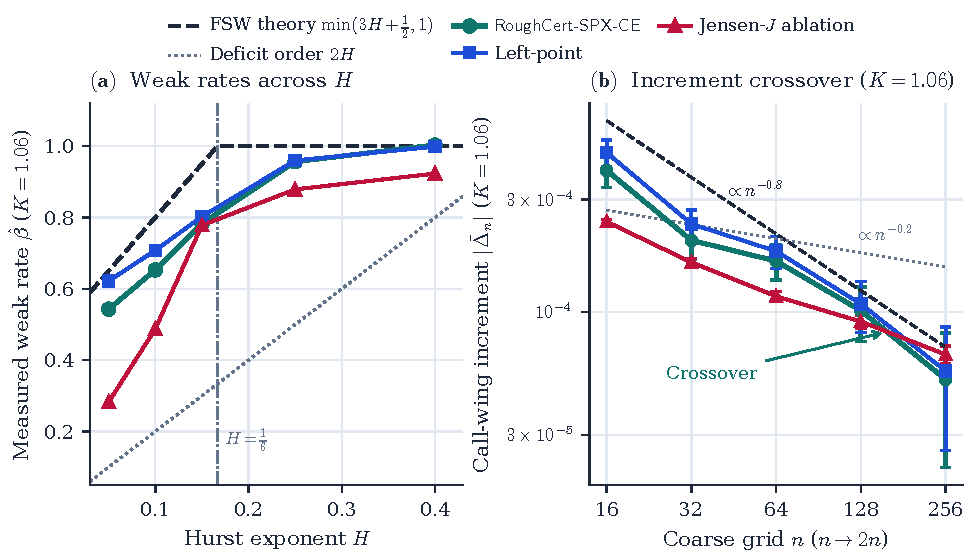
\includegraphics[width=\textwidth]{figures/fig_e5_weak_rates.pdf}
  \caption{Measured weak rates across $H\in[0.05,0.40]$ ($65{,}536$ paths, $n\in[16,512]$, $\eta=1.9$, $\rho=-0.9$). (a) Rate $\hat{\beta}$ at $K=1.06$ against $\min(3H+\tfrac12,1)$ \citep{FrizSalkeldWagenhofer2025} and the line $2H$. (b) Coupled increment magnitudes at $H=0.10$ with 95\% bars.}
  \label{fig:e5_rates}
\end{figure}

\begin{itemize}
  \item \emph{The FSW phase transition.} The left-point and \RCCE{} rates rise with $H$ and saturate near one for $H\ge 0.25$, as $\beta_{\mathrm{FSW}}$ predicts. At $K=1.06$ the left-point rates are $\EFiveLPHZeroFive$, $\EFiveLPHTen$, $\EFiveLPHFifteen$, $\EFiveLPHTwoFive$ and $\EFiveLPHForty$ for $H=0.05,0.10,0.15,0.25,0.40$, and the \RCCE{} rates are $\EFiveCEHZeroFive$, $\EFiveCEHTen$, $\EFiveCEHFifteen$, $\EFiveCEHTwoFive$ and $\EFiveCEHForty$. For $H\le0.15$ these single-strike rates lie below $\beta_{\mathrm{FSW}}(H)$, a pre-asymptotic effect on the tested grids, while the \RCCE{} strip-mean rate at $H=0.10$ ($\EFiveTenStripCE$) matches $\beta_{\mathrm{FSW}}(0.10)=0.80$.
  \item \emph{Support for Case~(ii) of Theorem~\ref{thm:bridge_envelope}.} For every tested $H\ge0.10$, all measured left-point and \RCCE{} rates (at $K=1.06$, at the money and on the strip mean) exceed the floor $\beta_{\min}(H)$, with margin at least $\EFiveMinMargin$ (check~C7b). At $H=0.05$ three rates fall below $\beta_{\min}(0.05)=\BetaMinZeroFive$ (\RCCE{} strip mean $\EFiveStripCEHZeroFive$, left-point strip mean $\EFiveStripLPHZeroFive$, \RCCE{} ATM $\EFiveATMCEHZeroFive$), so Case~(ii) envelopes are not supported there. Regime~B ($H=0.07$) lies between the tested values. Of all $\CaseTotalCount$ reference-envelope strikes in E1, E3, E4 and E6, $\CaseOneCount$ are in Case~(i), $\CaseTwoCount$ in Case~(ii) and $\CaseThreeCount$ are diagnostic (Supplementary Table~S3), so Case~(ii) carries most envelopes.
  \item \emph{Slower decay of the Jensen-$J$ ablation.} At $K=1.06$ the ablation's rates are $\EFiveJenHZeroFive$, $\EFiveJenHTen$, $\EFiveJenHFifteen$ and $\EFiveJenHTwoFive$ for $H=0.05,0.10,0.15,0.25$, below the \RCCE{} rates. The gap is negligible at $H=0.15$, where the ablation's ATM rate ($\EFiveATMFifteenJen$ against $\EFiveATMFifteenCE$) and strip-mean rate ($\EFiveStripFifteenJen$ against $\EFiveStripFifteenCE$) remain clearly lower; at $H=0.10$ its strip-mean rate is $\EFiveTenStripJen$ against $\EFiveTenStripCE$. Every resolved ablation rate exceeds $2H$, so the order suggested by the heuristic of Section~\ref{sec:jensen_pitfall} is not observed on these grids. Panel~(b) shows a crossover at $H=0.10$, $K=1.06$: on the coarsest grid the ablation's increment ($\EFiveTenJenCoarse$) is smaller than those of \RCCE{} ($\EFiveTenCECoarse$) and left-point ($\EFiveTenLPCoarse$), but it decays more slowly, and by $n=256$ the \RCCE{} point estimate ($\EFiveTenCEFine$) lies below the ablation's ($\EFiveTenJenFine$), with overlapping 95\% bars. A coarse-grid comparison alone would therefore favour the ablation despite its slower measured convergence.
\end{itemize}

\FloatBarrier
